\section{KeypointNet}

KeypointNet is a framework for end-to-end geometric reasoning that regresses the best set of category-specific 3D keypoints with their associated detectors, i.e., higher-dimensional generalized embeddings.
By definition, KeypointNet works for an image pair.
This framework estimates 3D pose by giving a differentiable goal that seeks the optimal set of keypoints to recover the relative pose of an item between two viewpoints.
Hence, KeypointNet allows for predicting geometrically and semantically consistent keypoints across viewing angles and instances of an object category by optimizing four loss functions.\\


\subsection{Loss functions}

The KeypointNet produces $N$ number of spatial probabilities for $N$ keypoints described by $g_i(u,v) \in \mathbb{R}^{W \times H}, \ac{s.t.} \ \sum_{u,v} g(u,v) = 1$.
The pixel spatial expectations is computed via continuous sampling method described by,

\begin{equation}
    [u_i, v_i]^T =  \left[ \displaystyle\sum_{u, v} g_i(u, v) * u , \  \displaystyle\sum_{u, v} g_i(u, v) * v \right]^T, \quad \ac{s.t.} \ g_i(u,v) \in \mathbb{R}^{W \times H}.
\end{equation}

\noindent Similarly, depth is computed as follows:
\begin{equation}
    d_i = \displaystyle\sum_{u, v} g_i(u, v) * d_i[u, v], \quad \ac{s.t.} \ d_i(u,v) \in \mathbb{R}^{W \times H}.
\end{equation}

The self-supervised training of this network is based on the following loss functions.






\subsubsection{Multiview Consistency Loss}

The multiview consistency loss function enforces the network to regress keypoint expectations at same the locations in an image pair.
Concisely, a keypoint in one image should project on a pixel location corresponding to a keypoint in another image.
To achieve this, pixels are projected to the camera frame using depth and intrinsic information. Using mutual transformation information
between two cameras, the pixels are further projected back to the pixel frame of the second camera. The loss is then the distance between the projected pixel location and
regressed keypoint's pixel location. \\

To make this formulation more intuitive, the originally proposed method is altered. Instead, of evaluating the keypoints in pixel frame, they are evaluated in the world frame.
The idealogy is that the object is fixed in the world datum and camera poses changes preserving the object coordinates in the world frame as depicted in Figure~\ref{fig:spat_exp} in page~\pageref{fig:spat_exp}.
The altered multiview consistency loss function is defined as,

\begin{equation}
    \mathcal{L}_{mvc} = \dfrac{1}{N} \displaystyle\sum^N_{i=1} \| W_A^i - W_B^i\|, \quad \ac{s.t.} \ W_{A, B} \in \mathbb{R}^{3 \times 1}.
\end{equation}





\subsubsection{Relative Pose Loss}

As the KeypoinNet produces $N$ number of keypoints, the keypoint locations together projected into the camera frame coordinates produces a 6D pose computed.
The relative pose loss function rearranges the keypoint locations in an image preserving the object's 6D pose in the viewpoint respective to the camera pose.
Additionally, this preserves the relative pose between two camera poses and relative pose generated from the keypoint locations in an image pair.\\

As per the original implementation of the KeypointNet, the authors discard the relative translation and expressed the relative pose
loss in form of chordal distance between two rotational matrices $ \in SO(3)$ using Frobenius-Norm \cite{bhatia2013matrix} as:

\begin{equation}
    \mathcal{L}_{pose} = 2 \arcsin \left( \dfrac{1}{2\sqrt{2}} \left\Vert \hat{R} - R \right\Vert_F \right) \quad,\ac{s.t.} \ R \in SO(3).
\end{equation}

Where, $\hat{R}$ is the groundtruth relative rotation of camera-a pose in the world frame and camera-b pose in the world frame and $R$ is the predicted relative rotation of regressed keypoints in an image pair.
The Frobenius norm yields the chordal distance in range $[0, 2 \sqrt{2}]$ which is normalized in the implementation.
The chordal distance formulation satisfying the triangle inequality condition involves ``\emph{some messy algebra}'' \cite{huynh2009metrics} as the operation $\hat{R} - R \notin SO(3)$. \\


To make this more geometrically intuitive, the poses $\in SE(3)$ are transported to $Riemannian$ $manifold$ \cite{lee2018introduction}.
$Riemannian$ $manifold$ is rich in geometry and differentiably smooth.
Instead, of expressing the distance in chordal form, `geodesic-distance' is chosen as it is smooth on for infinitesimally small trajectories on the manifold.
Here, the trajectory is defined as the distance to be covered such that the two rotation matrices align with each other.\\

The manifold geometry consists of two parts, i.e., a manifold and  a tangential plane tangential place $T(\mathcal{M}^p)$ represented as a tangential Euclidean space to the manifold, and the manifold space. the manifold space \( \mathcal{M}^p: p \in \mathbb{R}^{N^+}\).
Exp-maps and log-maps refer equation~\ref{eqn:logmap} are used to transport a vector on tangential plane to the manifold and vice versa.

\begin{equation}
    expmap: \mathfrak{so}(3) \rightarrow SO(3),
\end{equation}

\begin{equation}
    \label{eqn:logmap}
    logmap: SO (3) \rightarrow \mathfrak{so}(3).
\end{equation}

Here $r(\alpha) \in \mathfrak{so}(3) \in  T(\mathcal{M}^p)$ is a skew-symmetric matrix built from the axis angles $\alpha \in \mathbb{R}^3$ described as,

\begin{equation}
    r(\alpha) = \begin{bmatrix}
        0  & -z & y  \\
        z  & 0  & -x \\
        -y & x  & 0
    \end{bmatrix} \quad, \ac{s.t.} \ \alpha = [x, y, z]^T \in  \mathbb{R}^3.
\end{equation}

The object or camera's rotation in the dataset is represented as $SO(3)$.\\

The geodesic distance is a \emph{bi-invariant} metric on $SO(3)$ with range[0, $\pi$]:
\begin{equation}
    \label{eqn:geodesic}
    \mathcal{L}_{pose} = \dfrac{1}{\sqrt{2}} \| logmap(\hat{R}^T R) \|_F = \dfrac{1}{2} \| logmap(\hat{R}^T R) \|.
\end{equation}

The $\mathcal{L}_{pose}$ is substituted in the place of original loss function formulation.
The relative groundtruth rotation ($\hat{R}$) for the loss is computed as:

\begin{equation}
    \hat{R} = \hat{R}_{A \rightarrow B} = \hat{R}_A^{T} \ \hat{R}_B \quad,\ac{s.t.} \ \hat{R} \in SO(3).
\end{equation}

\noindent where, $\hat{R} = \hat{R}_{A \rightarrow B} \in \mathbb{R}^{3 \times 3}$ is the groundtruth relative rotation of camera-a pose in world $\hat{R}_A$ and camera-b pose in the world $\hat{R}_B$.
The camera poses are the extrinsic matrices available in the dataset. To compute the relative rotation $R$ of regressed keypoints
in an image pair, i.e., $X_A, X_B \in \mathbb{R}^{N \times 3}$ Kabsch's algorithm \cite{kabsch} is employed as follows:

\begin{equation}
    \mathcal{H} = (X_A - X_A^{mean})^T \ (X_B - X_B^{mean}) \quad,\ac{s.t.} \ \mathcal{H} \in \mathbb{R}^{3 \times 3}, \ X^{mean}_{A,B} = \overline{X}_{A,B}.
\end{equation}

\noindent where, $\mathcal{H}$ is the covariance matrix of the mean centered keypoint locations in the camera frame. To center the keypoint locations in the camera frame,
$X^{mean} \in \mathbb{R}^{1 \times 3}$ is computed along the dimension $N$ and each row in $X$ is subtracted with the mean.
The predicted relative rotation of keypoint locations in the image pair is computed as,

\begin{equation}
    R_B = V \begin{bmatrix}
        1 & 0 & 0          \\
        0 & 1 & 0          \\
        0 & 0 & det(V U^T)
    \end{bmatrix} U^T,
\end{equation}

where,

\begin{equation}
    U \Sigma V^T = SVD(\mathcal{H}).
\end{equation}

The term $det(V U^T)$ handles the reflection case while estimating the rotation matrix. In other terms it makes the $z$ rotation vector orthonormal to `$xy$'
rotation vectors such that it always points to the camera in the camera relative frame. This method to condition $z$ rotation vector produces gradients which allows neural networks
to be trained via backpropogation compared to using cross-product of vectors which does not produce gradients since the vector in the matrix is changed via inplace operation.









\subsubsection{Separation Loss}

Separation loss function penalizes cases where the distance between two keypoint locations is less than a specified margin ($\delta$).

\begin{equation}
    \mathcal{L}_{sep} = \dfrac{1}{N} \displaystyle\sum_i^N \displaystyle\sum_{j\neq i}^N max(0, \delta^2 - \| X_i - X_j \|^2).
\end{equation}







\subsubsection{Silhoutte Loss}

Silhoutte loss functions encourages the spatial probabilities of keypoints $g_i(u, v)$ to lie with the object silhoutte:

\begin{equation}
    \mathcal{L}_{obj} = \dfrac{1}{N} \displaystyle\sum^N_{i=1} -log \displaystyle\sum_{u, v} b[u, v] \ g_i(u, v).
\end{equation}

While training the network, the mask of the object is accessible. The mask values are sampled from the pixel locations $b[u, v] \in \{0, 1\}$. The mask information is only used
while training the network and is not using during the inference. If all the keypoints are regressed within the object silhoutte, the loss computes to zero.








\subsubsection{Variance Loss}

Variance loss function penalizes the spatial probabilities if they are broad in turn, encouraging peaky distribution.
The broader spatial probabilities brings in more uncertainty in the keypoint spatial expectation.
In turn, the loss function penalizes the uncertainty of the keypoint spatial expectation by shrinking the span of the spatial probabilities as depicted in Figure~\ref{fig:var_loss} in page~\pageref{fig:var_loss}.
Furthermore, in the Figure~\ref{fig:var_loss} in page~\pageref{fig:var_loss}, the x marks the keypoint spatial expectation. The left image illustrates the broader spatial probability of a keypoint bringing in more
uncertainty in the keypoint spatial location (expectation). The right image describes the peaky spatial probability of the keypoint encouraged by the loss function. \\

The variance loss functions is described as,

\begin{equation}
    \mathcal{L}_{var} = \dfrac{1}{N} \displaystyle\sum^N_{i=1} \displaystyle\sum_{u, v} g_i(u, v) \left\Vert \mathcal{G} - [u_i, v_i]^T \right\Vert^2,
\end{equation}

where $\mathcal{G}$ is the spatial grid of row and column indices described as,

\begin{equation}
    \label{eqn:spatial_grid}
    \mathcal{G}_{0ij} = \begin{bmatrix}
        0      & \dots  & 0      \\
        \vdots & \ddots & \vdots \\
        H      & \dots  & H
    \end{bmatrix}, \quad
    \mathcal{G}_{1ij} = \begin{bmatrix}
        0      & \dots  & W      \\
        \vdots & \ddots & \vdots \\
        0      & \dots  & W
    \end{bmatrix} \quad \quad,\ac{s.t.} \ \mathcal{G}  \in \mathbb{R}^{2 \times W \times H}.
\end{equation}

\begin{figure}[htb]
    \centering
    \caption{Variance loss function at work.}
    \label{fig:var_loss}
    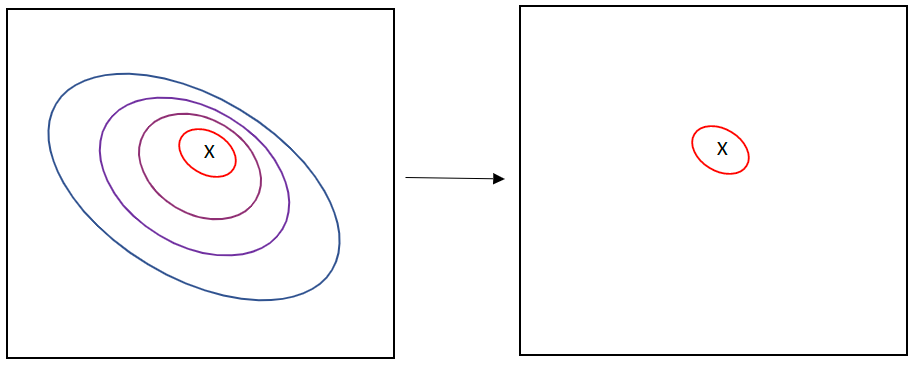
\includegraphics[scale=0.15]{images/keypointnet/var_loss.png}
\end{figure}

\subsection{Total Weighted-Sum Loss}

To train the network, all loss functions are weighed by their own specific weights inturn, signifying that one loss functions needs more priority than other loss functions.
The priority depends on the network architecture being used. Let's say if the multiview consistency loss is not converging, then the weights assigned to that particular loss function
are increased such that the multiview loss is further optimized by the network in the training phase. The total weighted loss function is the scalar product of the weights $W = [w_{mvc}, w_{pose}, w_{sep}, w_{obj}, w_{var}]^T $ and the individual
loss functions $ \mathcal{L} = [\mathcal{L}_{mvc}, \mathcal{L}_{pose}, \mathcal{L}_{sep}, \mathcal{L}_{obj}, \mathcal{L}_{var}]^T$ described as,

\begin{equation}
    \label{eqn: weighted_sum}
    \mathcal{L}_{Total} = < W, L > \quad,\ac{s.t.} \ \mathcal{L}_{Total} \in \mathbb{R} \ \& \ W,L \in \mathbb{R}^4.
\end{equation}

Here $W$ is a hyperparameter. The hyperparameter in this thesis implementation will be fixed by a trial-and-error process as other sampling or optimization process consumes a lot of time.

\subsection{Network Modification}

The \ac{ResNet} architecture will be used over originally proposed image segmentation based \ac{CNN} while preserving the part of architecture with
predicting depth and spatial probabilities of the keypoints to preserve the neural network architecture homogenity with \ac{DON} architecture.\\

Additionally, no pretrained orientation network is used to aid the KeypointNet breaking the symmetry of the objects as in \cite{suwajanakorn2018discovery}.
As per the proposed data augmentation in \cite{suwajanakorn2018discovery}, the data will not be scaled to a unit dimension preserving realistic
conditions of object in an environment for which the network will be trained for.



